\documentclass[11pt]{article}
\usepackage[UTF8]{ctex} % 支持中文编译（建议使用 XeLaTeX 编译）
\usepackage[margin=1in]{geometry}
\usepackage{amsmath,amssymb}
\usepackage{graphicx}
\usepackage{hyperref}
\usepackage{enumitem}
\usepackage{xcolor}
\usepackage{titlesec}
\usepackage{authblk}

\hypersetup{
    colorlinks=true,
    linkcolor=blue,
    urlcolor=blue,
    citecolor=blue
}

\titleformat{\section}{\large\bfseries}{\thesection.}{0.5em}{}
\titleformat{\subsection}{\normalsize\bfseries}{\thesubsection}{0.5em}{}

\graphicspath{{figs/}}

% =====================================================================
%  纪律一：正文每个数字必须能溯源（results JSON 或所引论文），没源不写。
%  纪律二：判据在跑实验之前写死，不随结果调整。负结果如实记录。
% =====================================================================

\title{\textbf{判别而非生成：面向冻结 JEPA 世界模型分层推演的物理引导边界检测}\\
\large \textbf{Judge, Don't Generate: Physics-Guided Boundary Detection for Hierarchical Rollout in Frozen JEPA World Models}}

\author{王嘉祺 (Jiaqi Wang)}
\affil{Eindhoven University of Technology \\ \texttt{j.wang11@student.tue.nl}}

\date{}

\begin{document}

\maketitle

\begin{abstract}
JEPA（联合嵌入预测架构）世界模型在潜空间（latent space）中学习显式的预测动力学并通过想象（imagination）进行规划，从而无需视觉-语言-动作（VLA）模型所依赖的语言监督，也无需扩散策略（diffusion policies）的迭代动作采样。然而，其核心短板在于长视界（long horizon）：推演（rollout）误差随步数逐步累积，现有模型的想象推演仅在数十步内保持可靠。现有的改进方案通常依赖训练分层结构：端到端的多层级架构虽然有效但训练代价高昂，而子目标生成器（subgoal generators）恰恰败在“生成”环节。在冻结的 LeWM 主干网络上，中等距离 PushT 任务中生成子目标的成功率仅为 $38.7\%$，低于扁平规划（flat planning）的 $52.7\%$，而真实（ground-truth）子目标的成功率可达 $73.3\%$。本文提出用“判别”替代“生成”：设计一个融合了物理先验与可学习参数的轻量级检测网络，直接读取冻结模型自身的潜变量，并判别当前推演是否仍处于同一动力学阶段（dynamical phase）。训练轨迹在离线状态下根据测量到的运动学事件（如接触、脱离接触和航向突变）进行分割，由此机械化提取的标签用于训练该检测器。在规划与执行阶段，检测到的边界共同决定了候选推演何时截断，以及闭环执行何时重新锚定（re-anchor）至真实观测，从而在每次相变处清零累积漂移。由于所有评估状态均取自模型自身的推演轨迹，不可达的伪造子目标在构造上即被排除在规划之外。主干网络保持完全冻结，适配新任务只需数小时的离线校准，无需端到端重训练。
\end{abstract}

\section{引言与相关工作 (Introduction and Related Work)}

联合嵌入预测架构（JEPA）通过预测下一时刻观测的表征（而非像素本身）来学习世界模型~\cite{lecun2022path,assran2023ijepa}。其学到的动力学是显式的：给定当前潜变量和动作，模型直接预测下一潜变量，使规划器能够完全在想象空间中评估候选动作序列。这规避了两项高昂代价：视觉-语言-动作模型所需的语言标注与任务演示，以及扩散策略所需的迭代采样。LeWorldModel (LeWM) 证明了此类模型可以从像素端到端稳定地完成训练~\cite{lewm2026}。

\begin{figure}[!t]
\centering
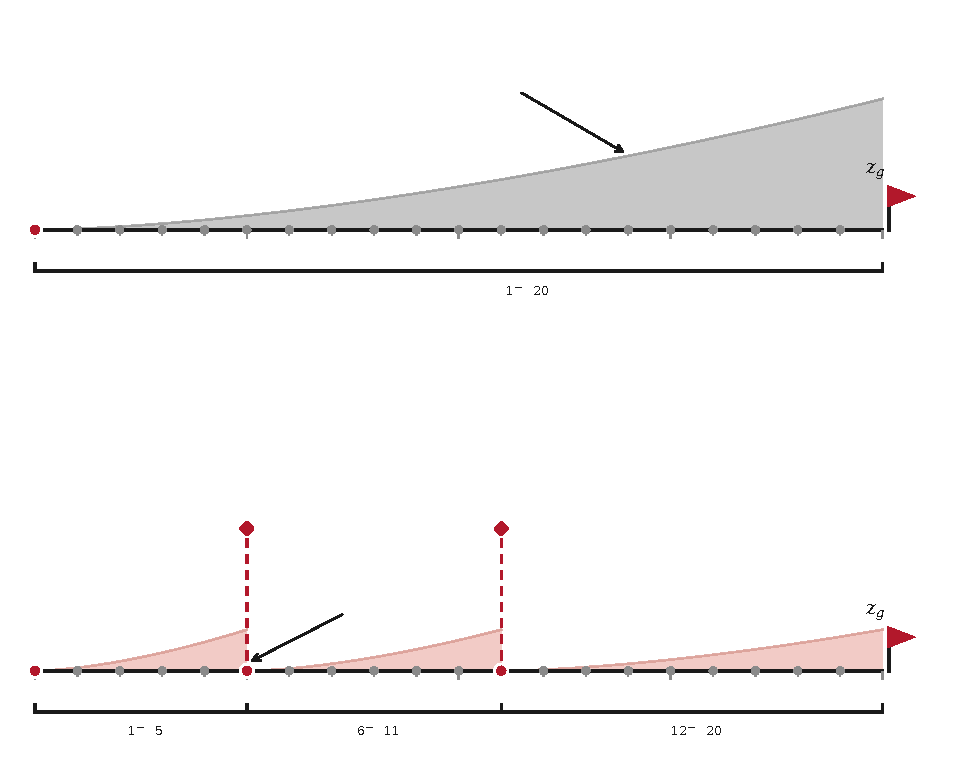
\includegraphics[width=0.96\textwidth]{rollout_flat_vs_seg_cn}
\caption{扁平规划与边界引导分割的对比。上：单次想象推演覆盖整个视界，全部动作联合优化，推演误差无重置地持续累积。下：检测器在物理相变边界处触发（边界检测 1、边界检测 2，虚线位置不等距）；每段以边界路标作为自身子目标、独立优化，执行在每个边界处重锚定至最新真实观测，累积漂移被清零。段长由检测到的事件决定，而非固定步长。}
\label{fig:rollout}
\end{figure}

然而，显式动力学也是其弱点所在。评估长视界候选序列意味着对单步模型进行自回归前向推演，预测误差在每一步不断累积，导致现有模型的想象推演仅在数十步内可信。在冻结的 LeWM 主干上，扁平规划的成功率从目标距离 $d=25$ 时的 $94.0\%$ 暴跌至 $d=75$ 时的 $18.0\%$~\cite{mindthegap2026}。

分层规划（Hierarchy）是标准解法：高层策略选择中间目标，使每个子问题都保持在底层模型的可信步长范围内。但在所有架构变体背后，决定成败的核心问题只有一个：\textbf{中间目标的潜变量从何而来？} 现有文献给出了三种答案，且每一种都暴露出了明确的诊断性缺陷。

\textbf{答案一：端到端训练分层架构} H-JEPA 堆叠了池化步长为 5、10 和 20 的多个层级并进行联合训练，将 AntMaze 的成功率从扁平规划的 $18.0\%$ 提升至 $73.3\%$~\cite{hjepa2026}。HWM 在共享潜空间中学习多个步长的模型，使粗粒度预测充当细粒度控制的中间目标~\cite{hwm2026}。性能增益是真实的，但其代价同样高昂：每一个新任务和每一种新本体（embodiment）都需要完整的端到端重训练。

\textbf{答案二：通过学习的高层策略生成子目标} Mind the Gap 冻结了预训练的底层模型，并在其上训练宏动作（macro-action）编码器与高层预测器~\cite{mindthegap2026}。在中等距离 PushT 任务上，生成子目标的得分仅为 $38.7\%$，低于同一冻结主干上扁平规划的 $52.7\%$，而来自数据集的真实子目标则高达 $73.3\%$。失败直接发生在“生成”环节：搜索过程挑出了高层模型打分很高、但偏离真实数据流形（off-manifold）的候选点，导致冻结的底层策略无法执行。作者的补救方案是将搜索范围严格限制在由真实轨迹编码的宏动作内，从而在两个最长距离上挽回了 $11.3$ 和 $14.7$ 个百分点，但这本质上等于放弃生成、转向数据。

\textbf{答案三：从数据中检索子目标} IMWM 通过检索演示轨迹来初始化并引导规划器的搜索方向~\cite{imwm2026}，上述限制宏动作搜索的修补方案也同属这一流派。检索虽然不会捏造虚假目标，但它只回答了“在附近哪里搜索”，却从未回答“哪些状态有资格作为路标（waypoints）”。此外，还有两条相关工作对执行节奏做在线调整：PACE 在预测的速度曲线上寻找低速过渡点作为重规划边界~\cite{pace2026}；AutoHorizon 则利用注意力权重估计模型自身的可靠范围，以动态设定执行步长~\cite{autohorizon2026}。

本研究占据了空缺的第四个生态位：\textbf{测量动力学边界，而非生成或检索空间路标}。任何任务的阶段结构（phase structure）都镌刻在接触、脱离和航向改变等物理事件中，而这些事件可以从训练轨迹中机械地直接读出。测量到的边界决定了推演在何处终止，以及闭环执行在何处从真实观测重新开始。整个方法中唯一的训练环节是一个融合了物理先验与可学习参数的轻量级校准网络，由离线测量生成的标签进行监督，因此它学到的是可跨任务实例泛化的“边界判别力”，而非僵化的硬编码规则。所有参与评估的状态均取自模型自身的推演轨迹，在构造上天然可达；每一项决策都归结为物理不变量与校准阈值的比对，确保全流程可审计，且仅需数小时即可完成新任务适配。

下文将依次阐述研究问题、核心方法、分阶段的工作计划，以及潜在风险与预期贡献。

\section{研究问题与科学假设 (Research Questions and Hypotheses)}

本提案不训练生成式高层策略，而是探究：在冻结的世界模型中，是否仅凭调控推演终止与重锚定（re-anchoring）的时机，就能复现分层规划的核心收益？我们把研究组织为四个可证伪的问题（RQ）与一项预注册的适用性预测（P1）：

\textbf{RQ1（边界触发重规划的可行性）} \textit{在冻结的 JEPA 主干上，于真实物理相变边界处终止并重锚定推演，能否显著优于扁平规划？} 我们首先通过真实分割上界（Oracle ground-truth segmentation）对此进行验证；在此处确立显著的性能优势是后续所有研究的先决条件。

\textbf{RQ2（归因分析：时机 vs.\ 频率，以及想象截断 vs.\ 执行重锚定）} \textit{第一，性能提升究竟源于将重规划对齐到物理边界，还是仅仅因为重规划更频繁？} 在严格匹配平均重规划频率的前提下，测量分割（Measured segmentation）必须击败等步长分割（Equal-stride segmentation）。\textit{第二，边界检测究竟在哪个环节起主导作用：是截断边界后不可靠的想象推演，还是在闭环执行中触发重锚定？} 我们将对这两种机制做系统对比。

\textbf{RQ3（相变边界的可观测特征）} \textit{哪种潜空间时间尺度分解与变点（change-point）统计量能够可靠地捕捉物理相变？} 我们不预设单一启发式指标，而是通过合成正对照实验（synthetic positive control）和留出集（held-out）边界 $F_1$ 分数，决定哪组估计器进入闭环规划测试。

\textbf{RQ4（可学习校准的价值）} \textit{在物理特征之上引入轻量级可学习读出层，其泛化能力是否优于固定解析阈值？} 可学习参数必须在三个迁移维度（留出噪声、未见任务布局、跨环境迁移）中至少两项上击败固定常数变体，否则将直接舍弃学习模块，回退至更简洁的解析方案。

\textbf{P1（预注册适用性预测）} 在 PushT 任务中，理想空间子目标之所以能带来巨大增益（$73.3\%$ vs.\ $52.7\%$），是因为它提供了中间空间路由（\textit{去哪里}）；而本文方法仅调控视界截断与重锚定的时机（\textit{何时停}），在方向引导上完全依赖全局目标潜变量。因此，本方法要求任务具备由明显时间尺度谱隙（spectral gap）分隔的不同动力学模态。我们预测：具有剧烈拓扑转换的导航任务（AntMaze）将获得显著收益；而接触密集的灵巧操作任务（PushT、Cube）由于克服瓶颈状态需要空间路标探索而非单纯消除累积漂移，其收益将相对有限。该预测在运行任何对比实验前正式锁定。

\section{研究方法 (Method)}

本方法固定了规划协议、标签生成机制、验收测试与对照实验设置。内部的谱估计与变点检测器则作为候选族列出，在进入闭环测试前通过严格的离线校准择优选用。

\subsection{边界引导的规划协议 (The boundary-guided planning protocol)}

规划过程沿用标准模型预测控制（MPC）框架，始终以最终目标潜变量 $z_g$ 作为唯一空间目标，唯一的修改在于用检测到的边界来调控推演评估与执行重锚定的时机（图~\ref{fig:rollout}）。由于提前截断想象推演需要在“减少累积误差”与“缩短前瞻视野”之间权衡，我们在协议中构建并对比两种核心机制：

\begin{enumerate}[leftmargin=*, nosep]
    \item \textbf{模式 A：全视界想象 + 仅执行重锚定（Full-Horizon Imagination with Execution-Only Re-anchoring）} 在规划阶段，候选动作序列在想象空间中推演至最大可信上限 $H_{\max}$（例如数十步），并直接按其末端状态到 $z_g$ 的潜空间距离打分，从而保留最远的前瞻视野以绕过非凸障碍。边界检测仅在闭环执行阶段介入：系统不再固定执行 $k$ 步，而是在真实观测流中一旦检测到相变边界（或达到 $H_{\max}$）便立即中止当前序列的执行，并从最新观测重新触发规划。
    \item \textbf{模式 B：边界截断想象 + 步长归一化打分（Boundary-Truncated Imagination with Normalized Scoring）} 在规划阶段，若某条候选推演在第 $h_b < H_{\max}$ 步触发了边界检测器，基于“跨过相变边界（如未建模碰撞或急转弯）后的开环预测不再可靠”这一前提，推演在 $h_b$ 步立即终止。为避免不同候选轨迹因终止步长 $h_b$ 不同而产生视界长度偏差（horizon-length bias），轨迹按其向目标潜变量推进的\textbf{单步归一化速率}进行打分，即 $\big(\|z_t - z_g\|_2 - \|z_{t+h_b} - z_g\|_2\big)/h_b$（同时以带折扣因子的终端距离作为消融对照）。闭环执行阶段则采用与模式 A 相同的事件触发重锚定机制。
\end{enumerate}

将模式 A 与模式 B 正面对比，能够直接回答一个核心问题：冻结 JEPA 模型在跨过物理边界后的潜空间预测，究竟提供了有益的远期引导，还是注入了有害的误导噪声？

\subsection{时间尺度测量 (Measuring time scales)}

为了区分快速瞬态波动与慢速任务进程，检测器需要对潜空间进行时间尺度分解。我们评估四类候选估计器：\textbf{(1)} 带初始正序列截断的自相关积分~\cite{geyer92}，计算简单但对编码器的任意坐标基底敏感；\textbf{(2)} 数据拟合线性算子的特征值，通过动态模态分解（DMD）及扩展 DMD（EDMD）~\cite{dmd,koopman_edmd,arbabi17} 转化为时间尺度 $\tau = -1/\ln|\lambda|$，对潜空间基底旋转保持不变；\textbf{(3)} 慢特征分析（SFA），直接提取慢变子空间~\cite{sfa}；\textbf{(4)} 在训练状态点处计算单步预测器雅可比矩阵（Jacobian）的谱分布，提供独立于轨迹采样策略的模型侧直接读数。在采信任何分解结果前，必须通过两道验证关卡：两种独立估计器必须在谱隙位置上达成一致；每个尺度组必须能在线性探针（linear probes）下解码出它所声称的物理要素，否则该冻结主干直接判定为不合格。

\subsection{相变边界检测 (Detecting boundaries)}

在提取出慢变与快变子空间后，我们评估三种候选边界信号：\textbf{(1)} 能量切换（Energy switching）：特定尺度组所占的潜变量增量能量比例偏离其段内基线，沿用经典变点检测（change-point detection）范式~\cite{page1954cusum,killick2012pelt,adams2007bocpd}；\textbf{(2)} 方向旋转（Direction rotation）：慢变子空间内连续步长增量之间的余弦相似度发生骤降，专门用于捕捉动能保持恒定但运动方向翻转的几何相变（如 AntMaze 走廊拐角）；\textbf{(3)} 算子漂移（Operator shift）：在滑动窗口上拟合的局部线性传播算子在谱距离上出现跳变~\cite{dmd,arbabi17}，直接反映局部动力学模态的切换。对于相变边界较为弥散的任务，我们保留基于无监督软聚类（soft phase-clustering）的备选方案。合成正对照与留出集 $F_1$ 分数将决定最终采用的边界信号。

\subsection{物理引导的可学习检测器 (The physics-guided learnable detector)}

为了在跨任务实例泛化的同时杜绝幻觉边界，检测器被设计为严格的两阶段混合架构：
\begin{enumerate}[leftmargin=*, nosep]
    \item \textbf{冻结的谱测量层：} 时间尺度常数以及快/慢子空间的投影矩阵完全通过 3.2 节的离线方法测定，并在后续全程保持严格冻结。
    \item \textbf{可学习的校准头：} 网络仅接收在潜变量增量上计算出的低维、物理可解释的不变量（各尺度组能量占比、慢子空间方向偏转角、局部算子距离）。一个紧凑的参数化模块负责学习读出权重与校准常数（窗口衰减系数、灵敏度指数与判定阈值），并由离线机械化提取的事件标签进行监督训练。
\end{enumerate}

三条铁律确保检测器扎根于物理：监督标签严格来自离线运动学测量，绝不使用网络自生成输出；谱基底由测量直接给出，不参与拟合；物理不变量的函数形式不可被梯度更新篡改。可学习变体与固定常数变体将进行正面对比，任何无法带来可观测迁移收益的学习参数都将被剔除。

\subsection{标签机制、验收标准与受控对比 (Labels, acceptance criteria, and controlled comparison)}

所有验证判据在闭环实验前预先锁定。参考边界标签从轨迹运动学特征中机械化提取（操作任务中取接触力脉冲与脱离事件；导航任务中取速度拐点与拓扑网格转换），绝不采用人工标注，并在每个环境中抽样 10 条轨迹进行目视核验。检测器的验收以严格步长容差内的留出集事件 $F_1$ 分数为准，且必须同时通过三项强制性健全性测试（sanity controls）：测量分割必须优于等步长分割；随机打乱阈值的检测器必须退化至随机水平；坍缩的常数潜变量必须输出零边界。

闭环对比实验在模式 A 与模式 B 下同时评估四种设置：\textbf{(1) 扁平规划（Flat planning）}、\textbf{(2) 等步长分割（Equal-stride segmentation）}、\textbf{(3) 测量分割（Measured segmentation）}，以及作为性能上界的 \textbf{(4) 理想真实分割（Oracle ground-truth segmentation）}。实验将在 AntMaze、PushT 和 Cube~\cite{hjepa2026} 三个环境中、跨越目标距离 $d \in \{25, 50, 75\}$，严格按照 Mind the Gap 评估协议~\cite{mindthegap2026} 运行，全面记录成功率、边界 $F_1$ 分数与实际规划耗时。

\section{分阶段工作计划与决策关卡 (Staged Work Plan and Decision Gates)}

本项目按关卡推进（gated execution plan）：每个阶段都是一道证伪过滤器，通过后才投入下一阶段的算力。任何关卡上的负面结果都作为实证发现如实记录并报告。

\textbf{阶段 0：基线复现与核验} 使用开源权重在全部三个环境及 $d \in \{25, 50, 75\}$ 距离设置下复现扁平规划基线，量化多随机种子下的方差分布。\textit{关卡：} 在推进后续研究前，必须彻底排查并解决与已发表基线之间的任何偏差。

\textbf{阶段 1：谱审计与预测预注册} 在各环境的训练数据集上测量潜空间时间尺度谱，通过线性探针验证子空间的物理语义，并正式锁定适用性预测（P1）。\textit{关卡：} 若所有环境均未呈现出可分离的谱隙，则直接作为表征诊断结论进行报告。

\textbf{阶段 2：自动化运动学打标} 从轨迹运动学中机械化提取参考边界标签，并在每个环境中人工抽检 10 条轨迹。\textit{关卡：} 若目视对齐失败，优先修正运动学提取启发式规则。

\textbf{阶段 3：检测器筛选与离线校准} 首先在合成切换线性动力学系统（switching linear dynamical system）上验证全部候选的时间尺度估计器（3.2 节）与边界信号（3.3 节），随后在真实轨迹上完成校准并评估留出集 $F_1$。\textit{关卡：} 唯有同时通过合成正对照与三项强制健全性测试的估计器，方可进入闭环规划。

\textbf{阶段 4：闭环规划归因实验（RQ1 \& RQ2）} 在三个环境、三种目标距离下运行四种规划设置，全面对比模式 A（仅执行重锚定）与模式 B（想象截断 + 执行重锚定）。首先运行 Oracle 真实分割以验证可行性上界（RQ1），随后开展同频率下测量分割与等步长分割的受控对比（RQ2）。

\textbf{阶段 5：泛化测试与消融分析（RQ4）} 训练可学习校准头，并在留出观测噪声、未见任务布局和跨环境迁移三个维度上与固定常数解析变体进行对比。若迁移增益不具备统计显著性，则舍弃可学习参数。

\textbf{阶段 6：快速适配基准测试} 将完整流水线封装为自动化校准脚本，在一个留出的任务变体上执行盲重校准，记录实际耗时（wall-clock runtime），以实证检验“数小时校准而非重训练”的核心主张。

\section{潜在风险与局限性 (Risks and Limitations)}

\textbf{泛化性与过拟合的权衡} 僵化的解析规则库只能识别校准集内出现过的相变幅度；反之，无约束的神经网络则极易过拟合潜空间中的伪影噪声。通过利用物理先验冻结谱投影与不变量函数形式、仅对低维决策头进行校准，本检测器能够在遵循相同底层物理规律的新边界配置上实现泛化。阶段 5 的三个迁移维度测试将对此进行直接检验。

\textbf{单段前瞻与全视界前瞻的权衡} 在模式 B 中，于第一个边界处截断想象虽然阻止了累积误差污染后续推演，但也限制了非凸环境中的前瞻视野（例如在 AntMaze 的 U 型弯中，走向拐角在短期内反而会拉大到目标的欧氏距离）。将模式 A 与模式 B 同时评估直接化解了这一风险：如果拓扑寻路确实需要全视界想象，而边界触发的重锚定足以稳定闭环执行，那么模式 A 恰好单独兑现这部分收益。

\textbf{任务适用边界} 边界触发式重规划要求任务的时间尺度谱存在可用谱隙，且更适用于“消除误差漂移”比“探索空间子目标”更关键的场景。通过在预注册假设（P1）下同时测试 AntMaze 与 PushT、Cube，无论是导航任务中的正向增益还是操作任务中的受限增益，都是界定“纯时序分层方法”适用边界的实证证据。

\textbf{主干网络的性能上限} 本文所有结论均以“冻结主干的潜空间已有效编码任务物理状态”为前提。阶段 1 的线性探针关卡显式过滤了退化的主干网络；由编码器层面的视觉域偏移（visual domain shift）导致的失效不在本研究讨论范围内。

\section{预期贡献 (Expected Contributions)}

\textbf{世界模型分层机制的解构} 我们直接检验以下核心假设：在冻结的 JEPA 世界模型中，分层规划的承重机制（load-bearing mechanism）在于推演终止的时机与闭环重锚定的节律，从而在机制上将“时序节奏调控”与“空间子目标生成”彻底解耦。

\textbf{确立“边界测量”第四技术路线} 我们补齐了分层世界模型规划的四条路线（端到端训练、子目标生成、数据检索、边界测量），并提供了横跨想象截断与执行重锚定双模式的受控对比基准。

\textbf{物理引导的边界校准架构} 我们提出了一种可审计的混合检测器架构，在解析变点规则与黑盒分类器之间架起桥梁，仅需轻量级离线校准即可将冻结的世界模型快速适配至新任务。

\bibliographystyle{plain}
\bibliography{refs}

\end{document}